\chapter{Programación del PLC}
\label{ch:progPLC}

Una vez montado el sistema, realizado el cableado eléctrico y verificado su
correcto funcionamiento de
manera manual, se procedió a la programación del \gls{plc}.

En el presente capítulo se describe tanto el algoritmo del programa de control,
como así también el lenguaje utilizado para implementar este algoritmo.
Además, se hará mención a las diferentes herramientas que ofrece el software
utilizado para el desarrollo y la implementación del programa en el \gls{plc}.

\section{Algoritmo}
\label{sec:Algoritmo}
Antes de realizar la programación en lenguaje Ladder, propio del \gls{plc},
se pensó en el algoritmo que incluya todas las tareas que el
controlador debe cumplir (gestión de alarmas, adquisición de parámetros,
control de la válvula, encendido y apagado de motores).
Se observa en el algoritmo (Alg. en adelante) \ref{img:algoritmo} la
solución propuesta.

\begin{algorithm}[!ht]
 \small
 \While{el tablero este energizado}{
  señal de PLC run\;
  adquisición de nivel, caudal y Set Point\;
  
  \If{Señal de parada de emergencia}{
   Apago los motores\;}
  
  \If{nivel > HHL}{
   alerta HHL y detención del sistema (si en modo automático)\;}
  \If{nivel < LLL}{
   alerta LLL y detención del sistema (si en modo automático)\;}
  
  \eIf{nivel > HL}{
   alerta de HL\;}{
   limpieza de alerta\;}
  
  \eIf{nivel < LL}{
    alerta LL\;}{
    limpieza de alerta\;}

  \If{deseo setear parámetros del controlador}{
    adquisición de nuevos valores Kp, Ti y Td\;}

  \eIf{deseo controlar el sistema manualmente}{
    \If{motor 1}{activo motor 1\;}
    \If{motor 2}{activo motor 2\;}
    Desactivo el PID y establezco la posición de la válvula de manera manual\;
    }
    {
    el sistema trabaja en modo automático\;
    \eIf{Planta en funcionamiento}{
	Enciendo los motores\;
	generación de consigna de la válvula en bloque del controlador PID\;
	constatar que el relevo térmico no se ha activado\;
	}{
	Apago los motores\;
    }
  }
}
 \caption{Tareas a cumplir por el controlador de manera secuencial.}
 \label{img:algoritmo}
\end{algorithm}

\section{Programación}
\label{sec:Programacion}
Se utilizó el programa Twido Soft, de Schneider Electric, para poder programar
el Alg. \ref{img:algoritmo} en lenguaje Ladder y posteriormente cargarlo en el
\gls{plc}.

\subsection{Breve descripción del lenguaje Ladder}

El lenguaje Ladder es muy utilizado en la programación de autómatas debido a
que es un lenguaje gráfico, basado en esquemas de tableros eléctricos de
lógica cableada \cite{bib:ApuntesPuglesiPLC}.
El principio de funcionamiento es sencillo: de acuerdo a una combinación
lógica de contactos en la entrada se obtiene una acción en la
salida.
Los elementos de entrada principales en Ladder son:

 \begin{itemize}
  \item Contacto normalmente abierto
  \item Contacto normalmente cerrado
  \item Conductor directo (representa un $1$ lógico)
 \end{itemize}

Los contactores pueden representar entradas/salidas de la
planta o valores en memoria.
Se combinan mediante acciones lógicas \verb|AND|, \verb|OR|, \verb|NOT|
(representadas mediante ``conductores'') y otros bloques de funciones (timers,
comparadores).
Se obtienen así nuevas señales, que pueden ser utilizadas para realizar
acciones de salida.

Las acciones de salida se representan como bobinas.
Las bobinas pueden estar aplicadas tanto a salidas físicas de la planta, como a
valores en memoria. Encontramos los siguientes tipos:

  \begin{itemize}
   \item \textbf{Bobina directa:} toma el valor lógico de la entrada.
   \item \textbf{Bobina inversa:} toma el valor lógico negado de la entrada.
   \item \textbf{Bobina set}: establece un valor de salida activo si encuentra
un valor lógico activo en la entrada. A diferencia de la bobina directa, si la
entrada se inactiva, el valor de salida se mantiene.
   \item \textbf{Bobina reset:} establece un valor de salida inactivo si
encuentra un valor lógico activo en la entrada.
   \item \textbf{Bloques de funciones:} permiten leer y escribir variables
numéricas, realizar bucles \gls{pid}, contadores, registros, etc.
  \end{itemize}
  
\subsection{Descripción del programa grabado en el PLC}

Cada una de las partes del programa se denomina \emph{RUNG} (escalón o
peldaño).
La ejecución de los peldaños es secuencial, comenzando por el \verb|RUNG 0|.
En cada peldaño se describen paso a paso las acciones que deseamos que
el controlador realice, de acuerdo al estado del sistema o las ordenes
recibidas desde el \gls{scada}.

La Fig. \ref{fig:ladder} muestra un diagrama de los diferentes peldaños de
nuestro programa de aplicación.
Se observa que la estructura secuencial del Alg. \ref{img:algoritmo} ha
sido respetada en los peldaños.


\begin{figure}
\centering
%\resizebox{0.8\textwidth}{0.9\textheight}{
\tikzstyle{every node}=[draw=black,thick,anchor=west,inner sep=2pt,minimum
size=1pt]
\tikzstyle{selected}=[draw=cyan,fill=cyan!30]
\begin{tikzpicture}[
  grow via three points={one child at (0.5,-0.7) and
  two children at (0.5,-0.7) and (0.5,-1.4)},   
  edge from parent path={(\tikzparentnode.south) |- (\tikzchildnode.west)}]
  \node (init) {Inicio del programa  }
    child { node {Inicialización} }
    child { node {Señal PLC run}    }
    child { node {Verificación de parada de emergencia}    }
    child { node {Adquisición de Nivel y Caudal}    }
    child { node {Gestión de alarmas HHL y LLL}    }
    child { node {Gestión de banderas de alarmas HHL y LLL}    }
    child { node {Gestión de alarmas HL y LL}    }
    child { node {Seteo de parámetros del controlador: Kp}    }
    child { node {Seteo de parámetros del controlador: Ti}    }
    child { node {Seteo de parámetros del controlador: Td}    }
    child { node {Seteo de parámetros del controlador: Set Point}    }
    child { node {Gestión de bandera de encendido y parada del sistema}    }
    child { node {Gestión de bandera de modo manual y automático}    }
    child { node {Gestión de motores si el sistema esta en modo automático}    }
    child { node {Encendido del Motor 1: Control manual y automático}    }
    child { node {Encendido del Motor 2: Control manual y automático}    }
    child { node {Controlador: PID}    }
    child { node {Valor de salida de la válvula}    }
    child { node {Gestión de señal de estado: manual o automático}    }
    child { node {Indicador del estado del Motor 1}    }
    child { node {Indicador del estado del Motor 2}    }
    child { node {Indicador de error en bombas}    }
    child { node {Gestión de bandera del sistema trabajando en modo normal}    }
    child { node {Limpieza de señal de parada de emergencia}    }
    child { node {Limpieza de alarmas}    };
\end{tikzpicture}
%}
\caption{Esquema de Rungs del programa Ladder de la planta de control de nivel}
\label{fig:ladder}
\end{figure}

\begin{itemize}
 \item Inicialización: Debido a una bandera se asegura el ingreso solo una vez a
 este peldaño del algoritmo. Se dan valores por defecto para las ganancias del 
 controlador y se fijan un Set Point al 50\%.
 \item Señal PLC run: Se envía una señal desde el \gls{plc} para saber que esta
 corriendo el programa.
 \item Verificación de parada de emergencia: Se leen las banderas de parada de 
 emergencia y se da la acción para parar los motores.
  \item Adquisición de nivel y caudal: Se leen las entradas analógicas para conocer
  el nivel del caudal y nivel.
  \item Gestión de alarmas: En estos escalones del programa lo que se hace es leer
  el valor de la palabra de memoria donde esta guardado el nivel del tanque, am partir
  de la comparación de este valor se muestran banderas en el \gls{scada} y si fuese 
  necesario se levanta la bandera para detener el sistema.
  \item Seteo de parámetros: En esta parte del programa se va a setear el parámetro
  correspondiente de acuerdo a lo que se escriba en la palabra \verb|MW1|.
  \item Encendido de los motores: A partir de la señal de encendido recibida desde el
  \gls{scada} o la señal de detención, se procede a activar una salida del lógica del
  \gls{plc}, esto sirve de señal visual para conocer desde el \gls{plc} el estado. 
  Si esta salida lógica que sirve como bandera esta activada, se activan las salidas
  lógicas correspondientes a los motores.
  \item Controlador \gls{pid}: En este peldaño se encuentra el bloque del controlador.
  La salida del mismo es el valor de apertura de la válvula.  
  La configuración de este bloque nos permite además de acuerdo a una bandera el manejo
  de manera manual de la válvula.
  \item Valor de salida de la válvula: Se lee el valor de salida de la válvula, este dato 
  nos sirve de retroalimentación a el \gls{scada}.
  \item Indicadores de estado del sistema: En estos peldaños se envía al software \gls{scada}
  el estado de los motores y si el sistema esta en modo manual o automático.
  \item Error en bombas: Una de las entradas digitales al \gls{plc} son la retroalimentación 
  recibida del rele de los motores. La lectura de esta señal nos indica si el motor esta 
  encendido. La retroalimentación no es tan rápida y en un primer momento, entonces 
  \item Sistema funcionando en modo normal: Si todo esta funcionando como esperamos, sin banderas
  de alarma se envía una señal en la palabra \verb|MW0| que indica que esta todo funcionando
  de manera correcta.
  \item Limpieza de alarmas: En este escalón se limpian las banderas de alarmas si eso es requerido
  por el usuario.
  
\end{itemize}


El \gls{plc} puede guardar información de diversa índole en memoria.
Estos valores en memoria pueden ser utilizados para modificar las salidas, a
modo de banderas.
También pueden guardarse valores numéricos, útiles para consignas,
ganancias o lecturas de sensores analógicos.
Se diferencian dos tipos de celdas de memoria:

\begin{table}[ht]
\renewcommand{\arraystretch}{1.3}
\centering
\begin{tabular}{c||c}
\hline
\bfseries Memoria & \bfseries Descripción\\
\hline \hline
\verb|M0|  & Bandera de inicialización\\
\verb|M1|  & Sistema Encendido/Apagado\\
\verb|M2|  & Sistema en modo Manual/Automático\\
\verb|M3|  & Error de Nivel\\
\verb|M4|  & Error de Motor\\
\verb|M4|  & Parada de emergencia\\
\hline
\end{tabular}
\caption{Banderas internas.}
\label{table:Banderasinternas}
\end{table}

\begin{itemize}
 \item \textbf{\gls{memory}:} tienen el formato \verb|Mx|, donde \verb|x| es un
número que comienza por $0$.
Son capaces de guardar un único bit.
Por esa razón, se utilizan como banderas internas del programa, que representan
distintos estados de la planta.
En la Tab. \ref{table:Banderasinternas} se pueden ver el nombre
de las banderas utilizadas en nuestro programa y sus funciones.
 \item \textbf{\gls{memoryWord}:} conocidas también como palabras, tienen el
formato \verb|MWx|, donde \verb|x| es un número que comienza por $0$.
Representan valores de $16$ bits de resolución. En ellos puede guardarse
información numérica en el rango $0$ a $65535$
(constantes, valores de lectura o escritura), o pueden utilizarse para guardar
hasta 16 banderas (bits).
Cabe destacar que las \gls{memoryWord} pueden ser leídas mediante el bus MODBUS
(ver \ref{sec:Comunicacion}).
En la Tab. \ref{table:mwBanderas} se muestran las \gls{memoryWord}
utilizadas como banderas, en tanto que en la Tab.
\ref{table:mwNumericos}
se muestran las \gls{memoryWord} utilizadas para guardar valores numéricos del
programa.
\end{itemize}


\begin{table}[!t]
\renewcommand{\arraystretch}{1.3}
\centering
\begin{tabular}{c||c||c||c}
\hline
\bfseries Tipo & \bfseries Word & \bfseries Bit & \bfseries Descripción\\
\hline \hline
Lect & \verb|MW0| & \verb|X0| & Señal Run PLC\\
Lect & & \verb|X1| & Alarma HHL\\
Lect & & \verb|X2|& Alarma LLL\\
Lect & & \verb|X3|& Alarma HL\\
Lect & & \verb|X4|& Alarma LL\\
Lect & & \verb|X5|& Error en motores\\
Lect & & \verb|X6|& Motor 1 encendido\\
Lect & & \verb|X7|& Motor 2 encendido\\
Lect & & \verb|X8|& Modo manual activado\\
Lect & & \verb|X9|& Modo automático activado y funcionando\\
Lect & & \verb|X10|& Planta funcionando sin errores\\
\hline
Esc & \verb|MW1| & \verb|X0|& Switch Encender(1)/Apagar(0)\\
Esc & & \verb|X1|& Manual(1)/Automático(0)\\
Esc & & \verb|X2|& Cambiar parámetros PID\\
Esc & & \verb|X3|& Cambiar Set Point\\
Esc & & \verb|X4|& Manual(0)/Default(1)\\
Esc & & \verb|X5|& Encender M1 (manual)\\
Esc & & \verb|X6|& Encender M2 (manual)\\
Esc & & \verb|X7|& Limpiar errores\\
Esc & & \verb|X8|& Parada de emergencia\\
Esc & & \verb|X9|& Limpiar señal de parada de emergencia\\
\hline
\end{tabular}
\caption{Memory Words utilizadas como banderas.}
\label{table:mwBanderas}
\end{table}

\begin{table}[!t]

\renewcommand{\arraystretch}{1.3}
\centering
\begin{tabular}{c||c||c}
\hline
\bfseries Tipo & \bfseries Word  & \bfseries Descripción\\
\hline \hline
Lect & \verb|MW2|  & Lectura DP cell nivel (era \verb|MW1|)\\
Lect & \verb|MW3|  & Lectura DP cell caudal\\
Lect & \verb|MW4|  & Valor Kp\\
Lect & \verb|MW5|  & Valor Ti\\
Lect & \verb|MW6|  & Valor Td\\
Lect & \verb|MW7|  & Valor de lectura del SP (era \verb|MW2|)\\
Lect & \verb|MW8|  & Valor de lectura de la válvula (era \verb|MW7|)\\
\hline
Esc & \verb|MW9| & Valor de escritura de la válvula (manual) (era 
\verb|MW15|) \\
Esc & \verb|MW10|  & Valor de escritura del SP \\
Esc & \verb|MW11|  & Valor de escritura Kp \\
Esc & \verb|MW12|  & Valor de escritura Ti \\
Esc & \verb|MW13| & Valor de escritura Td \\
\hline
\end{tabular}
\caption{Memory Words utilizadas para almacenar valores numéricos.}
\label{table:mwNumericos}
\end{table}

Finalmente, se detallan a continuación las entradas y salidas al \gls{plc} de 
la planta.
Descriptas en la Sec. \ref{subsec:plc}, permiten al
controlador relevar variables de la planta y aplicar acciones de control. 
En la Tab. \ref{table:entradassalidas} se muestran las
entradas/salidas tanto analógicas como discretas.
Cabe destacar que la salida \verb|Q0.7| se utilizó para obtener un indicador
visual del estado de la planta en el plc.
Esta salida no está conectada.

En el anexo \ref{anexo:programaLadder} se puede
observar el programa en
lenguaje Ladder completo y todos los parámetros del \gls{plc}, en el
software Twido Soft.

\begin{table}[!t]

\renewcommand{\arraystretch}{1.3}
\centering
\begin{tabular}{c||c||c}
\hline
\bfseries Tipo & \bfseries Memoria & \bfseries Descripción\\
\hline \hline
Salida & \verb|Q0.0|  & Encendido motor 1\\
Salida & \verb|Q0.1|  & Encendido motor 2\\
Salida & \verb|Q0.7|  & Señal de encendido de la planta en modo automático\\
Salida & \verb|I0.0|  & Retroalimentación desde el relevo térmico motor 1\\
\hline
Entrada & \verb|I0.1|  & Retroalimentación desde el relevo térmico motor 2\\
Entrada & \verb|IW0.1.0|  & Señal analógica de nivel\\
Entrada & \verb|IW0.1.1|  & Señal analógica de caudal \\
Entrada & \verb|QW0.1.0|  & Señal analógica de salida de apertura de la válvula
\\
\hline
\end{tabular}
\caption{Entradas y salidas al PLC}
\label{table:entradassalidas}
\end{table}

\section{Controlador PID}
\label{sec:controladorpid}
\glsreset{pid}

El algoritmo utilizado en la planta de control de nivel, implantado en el
\gls{plc}, es de tipo \gls{pid}.
En un controlador \gls{pid} la acción correctiva es la suma de tres valores, a
saber:

\begin{itemize}
 \item Proporcional al error.
 \item Proporcional a la integral del error respecto del tiempo.
 \item Proporcional a la derivada del error respecto del tiempo.
\end{itemize}
La constante de proporcionalidad para cada caso se conocen como ganancias del
controlador ($K_p$, $T_i$ y $T_d$).

El \gls{plc} utilizado ofrece hasta 14 bloques \gls{pid}, del cual utilizamos
sólo uno.
Se muestran en la Tab. \ref{table:controladorpid} los valores utilizados para
la configuración del controlador PID.
Cada bloque \gls{pid} tiene dos modos de trabajo.
\begin{itemize}
 \item \textbf{Modo automático:} conociendo los valores de las ganancias, el
set point y la variable controlada, realiza el algoritmo de \gls{pid} y entrega
un valor de la variable manipulada en salida.
En nuestro caso, la variable manipulada es la apertura de la válvula.
La variable controlada y el set point corresponden a los valores de nivel
presente en el tanque y deseado, respectivamente.
 \item \textbf{Modo manual:} permite anular el controlador, enviando un valor
manual a la variable controlada.
Podemos así controlar la apertura a la válvula cuando se
trabaja en modo manual desde el \gls{scada}.
 \item \textbf{Parada de emergencia:} se previó como un sistema de parada de emergencia.
 Como se explicara en el capitulo \ref{ch:scada} esta previsto un
 botón exclusivo para esta acción. Este debe detener
 los motores en no importa que modo de funcionamiento de la planta. Al accionar el 
 botón desde el software \gls{scada}, se levanta una bandera en el \gls{plc}
 que da la señal de detener los motores. Luego de solucionar el posible inconveniente
 que desencadeno la parada de emergencia de la planta se debe enviar una señal 
 al \gls{plc} para limpiar la bandera de señal de emergencia: Rehabilitar al 
sistema para su funcionamiento normal.
\end{itemize}

\begin{table}[!t]
\renewcommand{\arraystretch}{1.3}
\centering
\begin{tabular}{c||c||c}
\hline
\bfseries Tipo & \bfseries Word  & \bfseries Descripción\\
\hline \hline
Variable Manipulada & \verb|IW1.0|  & Nivel actual del tanque controlado\\
Consigna & \verb|MW2|  & Nivel deseado\\
Ganancia PID & \verb|Kp|  & Ganancia proporcional\\
Ganancia PID & \verb|Ti|  & Ganancia integral\\
Ganancia PID & \verb|Td|  & Ganancia derivativa\\
Variable controlada & \verb|QW1.0|  &  Apertura de la válvula (automático)\\
Bandera & \verb|M2|  & 1: Modo manual, 0: Modo automático \\
Valor manual & \verb|MW15|  & Apertura de la válvula (manual)\\
\hline
\end{tabular}
\caption{Configuración del PID.}
\label{table:controladorpid}
\end{table}

\subsection{Determinación de las ganancias}

Para poder determinar las ganancias del controlador se decidió seguir el método
de Ziegler–Nichols.
Se trata de una serie de reglas basadas en la respuesta experimental
del sistema.
Estas reglas son aplicables a sistemas de primer orden, donde no se conoce con
precisión el modelo matemático del sistema \cite{bib:Ogata}.

Se presentan dos métodos:
\begin{itemize}
 \item \textbf{Primer método:} se obtiene experimentalmente la respuesta de la
planta a una entrada en escalón.
 La respuesta puede ser caracterizada por dos constantes, el tiempo de retardo
$L$ y una constante de tiempo $T$.
Se obtienen las constantes dibujando
una recta tangente al  punto de inflexión de la curva de la respuesta del
sistema, como muestra la Fig. \ref{fig:primermetodo}.
Luego, se calculan las ganancias utilizando la Tab. \ref{tab:valorganancias}.

 \item \textbf{Segundo método:}
 este método comienza su análisis con un controlador puramente proporcional.
 Se incrementa  la ganancia proporcional desde cero hasta un valor $Kp_{cr} $
donde la respuesta del  sistema presenta oscilaciones permanentes como en la
Fig. \ref{fig:segundometodo}.
 Mediante los valores de $Kp_{cr} $ y $P_{cr}$ pueden calcularse las ganancias
del controlador.
Nuevamente, las ganancias pueden ser calculadas utilizando la Tab.
\ref{tab:valorganancias}.
\end{itemize}

\begin{figure}[ht]
 \centering
 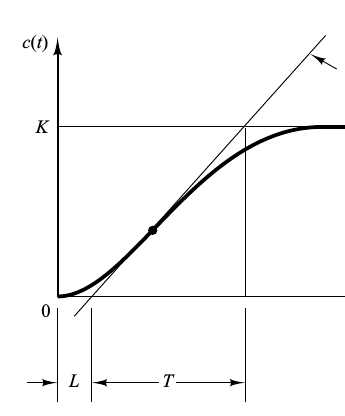
\includegraphics[scale=0.5]{Cap4-ProgramacionPLC/images/primermetodo.png}
 \caption{Respuesta del sistema a un escalón \cite{bib:Ogata}.}
 \label{fig:primermetodo}
\end{figure}

\begin{figure}[ht]
 \centering
 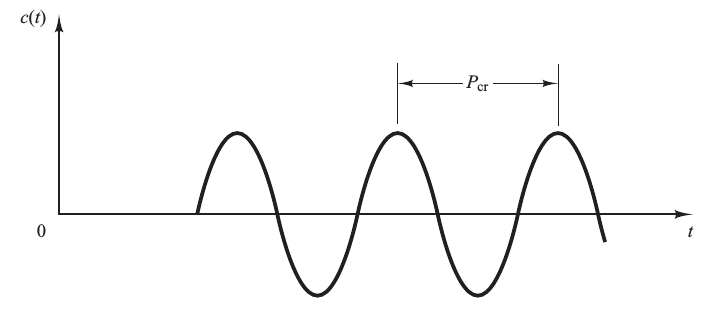
\includegraphics[scale=0.5]{Cap4-ProgramacionPLC/images/segundometodo.png}
 \caption{Oscilación permanente del sistema \cite{bib:Ogata}.}
 \label{fig:segundometodo}
\end{figure}

\begin{table}[!t]
\renewcommand{\arraystretch}{1.3}
\centering
\begin{tabular}{c||c||c |c}
\hline
\bfseries Método & \bfseries Kp  & \bfseries Ti & \bfseries Td\\
\hline \hline
Primero &  $ 1.2 \, {T}/{L}$ & $2 \, L $ & $ 0.5 \, L $\\
\hline
Segundo &  $0.6 \,Kp_{cr}  $ & $ 0.5 \, P_{cr}$ & $0.125 \, P_{cr} $\\
\hline
\end{tabular}
\caption{Valor de las ganacias según el método Ziegler–Nichols.}
\label{tab:valorganancias}
\end{table}

\subsubsection{Cálculo de ganancias en nuestra planta}

Para nuestro trabajo se optó por el segundo método de los presentados
anteriormente, es decir, poniendo al sistema en oscilación permanente en bucle
cerrado.

\paragraph{Sin tiempo muerto}

Se colocó a la planta en oscilación, como muestra la Fig.
\ref{fig:oscilacionperm}.

\begin{figure}[ht]
 \centering
 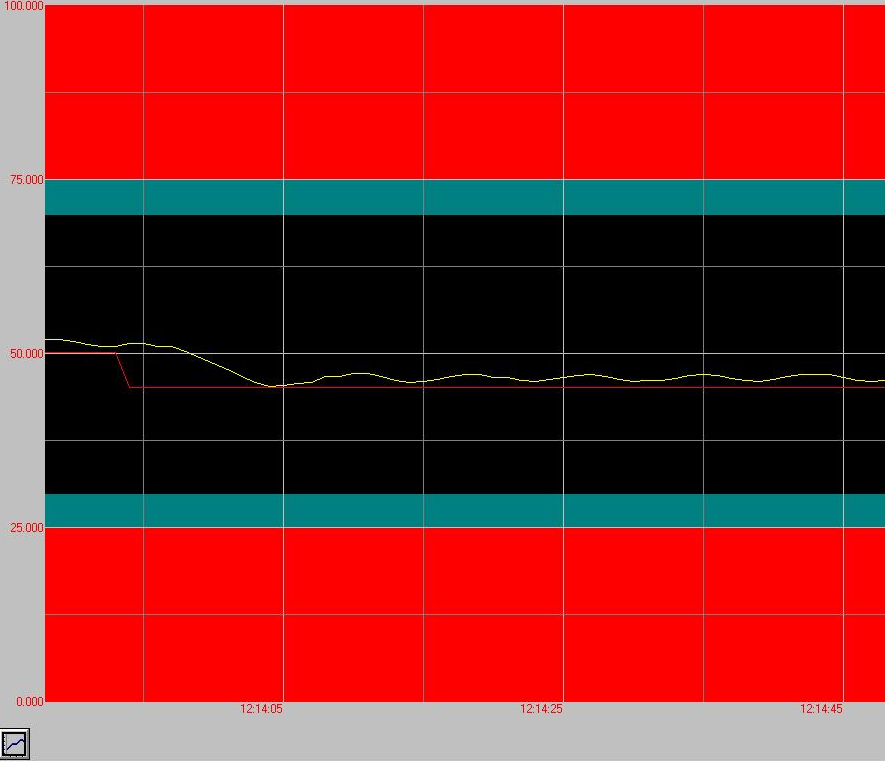
\includegraphics[scale=0.4]{Cap4-ProgramacionPLC/images/oscperm.png}
 \caption{Nivel de la planta en oscilación, sin tiempo muerto.}
 \label{fig:oscilacionperm}
\end{figure}

Se obtuvieron los siguientes valores de $Kp_{cr} $ y $P_{cr}$.

\begin{itemize}
 \item $Kp_{cr}$:
 $60$
 \item $P_{cr}$:
 $8 s$
\end{itemize}

A partir de estos datos se obtuvieron los valores de las ganancias:

\begin{itemize}
 \item $K_p $: $36$
 \item $T_i $: $4$
 \item $T_d $: $1$ 
\end{itemize}

En la Fig. \ref{fig:controlado} se puede apreciar el seguimiento de la
consigna de nivel en la planta, funcionando con estos valores de ganancias.

\begin{figure}[ht]
 \centering
 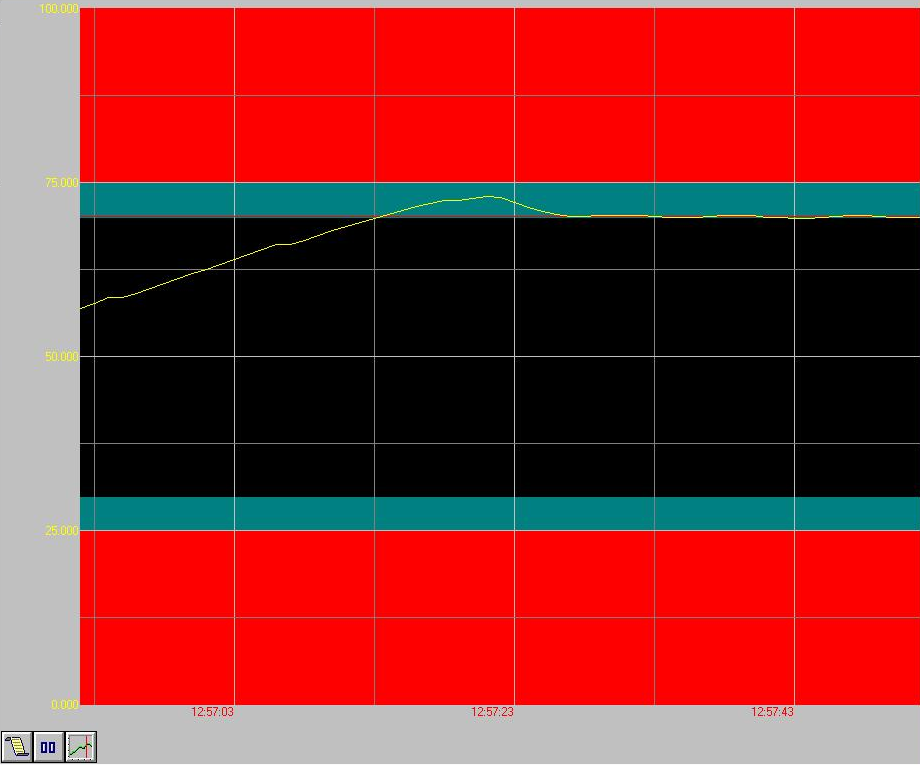
\includegraphics[scale=0.4]{Cap4-ProgramacionPLC/images/controlado.png}
 \caption{Nivel de la planta controlada, sin tiempo muerto.}
 \label{fig:controlado}
\end{figure}


\paragraph{Con tiempo muerto}

Nuevamente, se coloca la planta en oscilación como muestra la Fig.
\ref{fig:oscilacionpermtd}.
Se obtuvieron los siguientes valores de los parámetros.

\begin{figure}[ht]
 \centering
 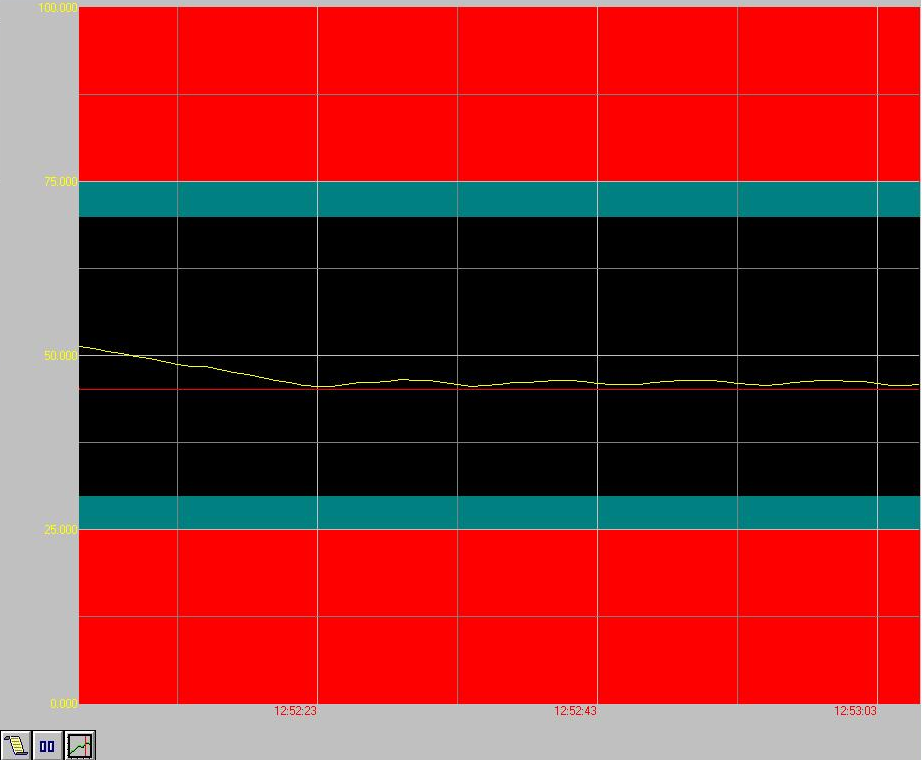
\includegraphics[scale=0.4]{Cap4-ProgramacionPLC/images/oscpermtd.png}
 \caption{Nivel de la planta en oscilación, con tiempo muerto.}
 \label{fig:oscilacionpermtd}
\end{figure}

\begin{itemize}
 \item $Kp_{cr}$:
 $120$
 \item $P_{cr}$:
 $10 s$
\end{itemize}

A partir de estos datos se obtuvieron los valores de las ganancias
para la planta, trabajando con tiempo muerto:

\begin{itemize}
 \item $K_p $: $72$
 \item $T_i $: $5$
 \item $T_d $: $1.25$
\end{itemize}

En la Fig. \ref{fig:controladotd} se puede apreciar el seguimiento de consigna
de nivel, utilizando el circuito de tiempo muerto.

\begin{figure}[ht]
 \centering
 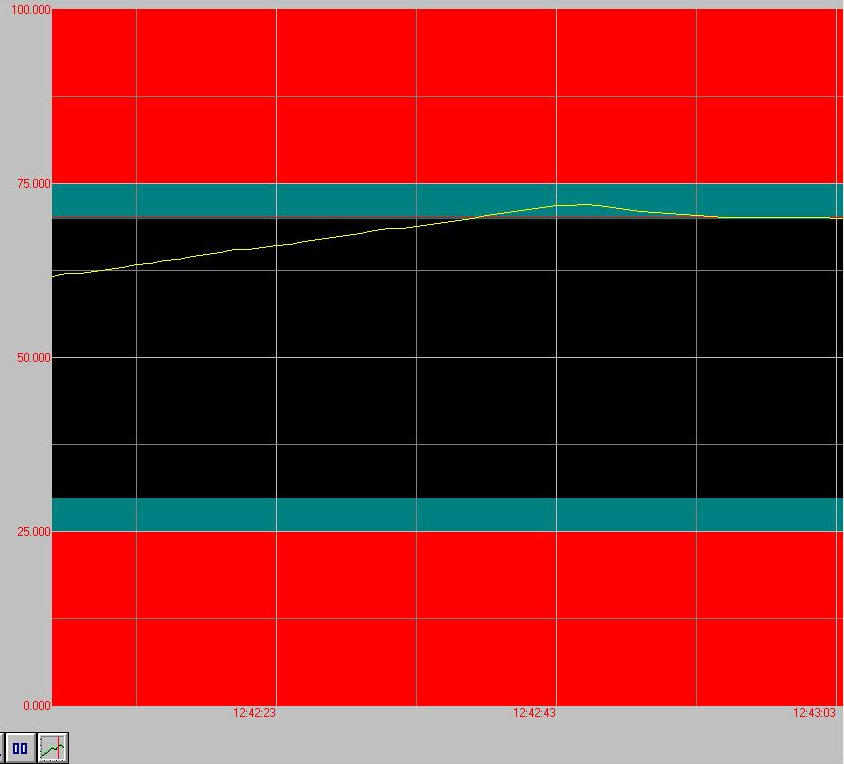
\includegraphics[scale=0.4]{Cap4-ProgramacionPLC/images/controladotd.png}
 \caption{Nivel de la planta controlada, con tiempo muerto.}
 \label{fig:controladotd}
\end{figure}

Queda así validada la sintonía del bucle \gls{pid} en el controlador.

\section{Comunicación}
\label{sec:Comunicacion}

Tal como se mencionó anteriormente, mediante MODBUS sólo se puede tener acceso 
a las \gls{memoryWord} (palabras) del \gls{plc}.
Para interactuar con la planta debieron definirse ciertas palabras, que
permiten realizar acciones en el sistema y conocer el estado del mismo.
Por simplicidad, se optó por utilizar dos grupos de palabras bien
diferenciadas:
\begin{itemize}
 \item \textbf{Palabras de lectura:} pueden ser leídas por la computadora de
control mediante MODBUS. En las palabras de lectura agruparemos aquellas
banderas de estado (motores encendidos, alarmas) y las palabras con valores
numéricos de lectura (mediciones de nivel, caudal, valor presente de set point
y de ganancias del controlador).
 \item \textbf{Palabras de escritura:} pueden ser escritas por la computadora
de control. Aquí se agrupan valores numéricos que pueden ser cambiados (set
point, ganancias) y banderas para modificar el estado de la planta (encenderla,
seteo en modo manual, encendido de las bombas).
\end{itemize}

Destacamos que en algunos casos (por ejemplo, set point) tenemos tanto palabras
de lectura o escritura.
Esto se debe a que estas variables, importantes para el funcionamiento de la
planta, deben ser modificadas solamente bajo solicitud expresa del usuario
, es decir, mediante la seteo de la bandera que permita tal modificación.

La Tab. \ref{table:mwBanderas} presenta dos palabras de dieciséis
bits, \verb|MW0| y \verb|MW1|, la primera de ella presenta bits de lectura, en
donde se
refleja el estado del la plata, mientras que la segunda palabra tiene bits de
de escritura para enviar acciones de control.

Por otro lado la Tab. \ref{table:mwNumericos} nos presenta
las palabras restantes, utilizadas en el programa para
almacenar valores numéricos.
La primer parte de la tabla muestra las palabras de solo lectura (valores que
presentan las variables del sistema), mientras que en la
segunda parte muestra las palabras de escritura (reservadas al cambio
de los parámetros del sistema).

\section{Depuración (Debug)}
\label{sec:Debug}

Una vez finalizada la programación y antes de vincular el \gls{plc}
al \gls{scada}, se realizaron una serie de pruebas correspondientes para
validar el correcto funcionamiento del programa.

El software Twido Soft permite realizar la depuración
en tiempo de ejecución, observando el estado de las diferentes variables
de la planta.
La animación colorea las bobinas y contactores que están activos, permitiendo
identificar problemas lógicos en el programa.
Además, podemos observar el valor de las entradas y salidas, detectando así
errores en la instrumentación y/o en los actuadores.

En la Fig. \ref{img:twidosoftdebug} se observa el módulo \emph{Tablas
de Animación} de Twido Soft.
Mediante este módulo, se puede forzar el estado de algunas bobinas y cambiar el
valor de las palabras en memoria.
Podemos así generar situaciones características que encontraremos durante la
operación de la planta.
Podemos citar:

\begin{figure}[ht]
	\centering
	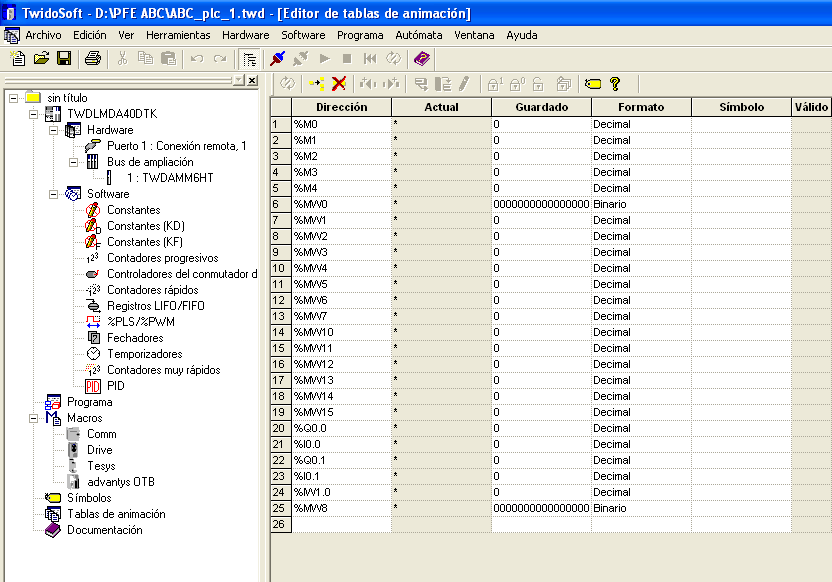
\includegraphics[width=.8\textwidth]
	{Cap4-ProgramacionPLC/images/twidosoftdebug.png}
	\caption{Esquema de la división del tiempo}
	\label{img:twidosoftdebug}
\end{figure}

\begin{itemize}
 \item \textbf{Lectura de las variables analógicas:}
 se constato que los valores recogidos con las entradas analógicas sean
congruentes con el valor que se observa en las DP cell.

  \item \textbf{Encendido y parada del sistema en modo automático:} cambiando
la palabra \verb|MW1|, se verificó el correcto arranque del sistema en modo
automático, con un Set Point preestablecido.

 \item \textbf{Correcto funcionamiento del Controlador \gls{pid}:}
 se verificó el funcionamiento de la planta al cambiar el Set Point.
Se verifican así las ganancias del controlador, como así también el correcto
funcionamiento de la válvula de control.

 \item \textbf{Correcto funcionamiento de las alarmas y paradas de emergencia:}
 se forzó un estado anormal en el sistema para verificar el funcionamiento de
las alarmas y paradas de emergencia, en una situación crítica. Por ejemplo, se
estableció un set point superior a HHL.
 Se verifica cambio en la palabra \verb|MW0| al sobrepasar HL.
 Luego, al sobrepasar HHL, no solo se constato el cambio en la
 palabra \verb|MW0|, sino que además se verificó la correcta detención de la
planta (bandera \verb|M3|).
 De la misma manera se verificaron las alarmas y paradas por bajo nivel.
 
 \item \textbf{Seteo de parámetros:}
 hasta este momento los valores de las ganancias del controlador eran las
establecidas por defecto durante el arranque del controlador.
 En esta prueba, se verificó el cambio de las ganancias del \gls{pid} en tiempo
de ejecución, modificando la palabra \verb|MW1| y la
correspondiente palabra de acuerdo al valor que se desee modificar.
 
 \item \textbf{Control del sistema en modo manual:}
 modificando la palabra \verb|MW1| se puso el sistema de modo manual.
 Se cambió la apertura de la válvula y se verificó el arranque de cada motor
por separado.
 
 \item \textbf{Parada de emergencia por error en el funcionamiento de los
motores:} por ultimo se forzó nuevamente al sistema a una situación extrema, en
la que uno de los motores se detiene por sobrecorriente (debido al rotor
atascado o sobrecalentamiento).
 El sistema se detiene (bandera \verb|M4|) y la palabra \verb|MW0| acusa que el
motor no está encendido.
\end{itemize}
